\documentclass[11pt]{article} % For LaTeX2e
\usepackage{manuscript, palatino}
\usepackage{graphicx}
\usepackage{amsfonts, amsmath}
\usepackage{algorithm, algpseudocode}%

\title{Anxiety: a decision-theoretic perspective}

\author{
Samuel Zorowitz \\
Princeton Neuroscience Institute\\
Princeton University\\
Princeton, NJ 08540 \\
\texttt{zorowitz@princeton.edu} \\
\And
Nathaniel Daw \\
Princeton Neuroscience Institute\\
Princeton University\\
Princeton, NJ 08540 \\
\texttt{ndaw@princeton.edu} \\
}

% The \author macro works with any number of authors. There are two commands
% used to separate the names and addresses of multiple authors: \And and \AND.
%
% Using \And between authors leaves it to \LaTeX{} to determine where to break
% the lines. Using \AND forces a linebreak at that point. So, if \LaTeX{}
% puts 3 of 4 authors names on the first line, and the last on the second
% line, try using \AND instead of \And before the third author name.

\newcommand{\fix}{\marginpar{FIX}}
\newcommand{\new}{\marginpar{NEW}}

\begin{document}

\maketitle

\begin{abstract}
To be filled in
\end{abstract}

\keywords{
reinforcement learning; avoidance; anxiety
}

\startmain

\section{Introduction}
Many psychiatric disorders involve distortions in models of the external world
and, correspondingly, aberrations of learning and decision making. As a normative
framework, decision theory allows us to describe and pose quantita­tive questions
about optimal and approximately optimal choice behavior \cite{DayanDaw2008} and
is, therefore, a critical tool for modeling, understanding, and predicting the
psychological and neurobiological mechanisms responsible for the abnormalities
observed in psychiatric behavior \cite{HuysDawDayan2015}. Many recent investigations
employing this approach have provided important insights into psychiatric symptoms,
including anhedonia in major depression \cite{Rutledge2017}, mood instability
in bipolar disorder \cite{EldarNiv2015, EldarDolanNiv2016},  habitual decision
making in disorders of compulsivity \cite{gillan2016}, and hallucinations in
schizophrenia \cite{powers2017, corlett2018}.

Anxiety disorders (generalized anxiety disorder, social anxiety disorder, panic
disorder, obsessive-compulsive disorder) represent the most common family of
psychiatric disorders (citation). Despite the differences in the content of worry,
all anxiety disorders share two core features: pessimistic inference and excessive
avoidance. Pessimistic inference describes a tendency to appraise threatening
situations as more frequent and/or more severe than they objectively are. This has
been reliably observed experimentally, as in fear conditioning wherein individuals
with anxiety exhibit exaggerated fear towards safe cues (CS-) and extinguished
threatening cues \cite{lissek2005, Duits2015}, and clinically, through self-report
(pick 3 citaitons). Excessive avoidance describes the corresponding tendency for
individuals with anxiety to consistently flee or avoid threatening situations.
Avoidance is often chosen even at the expense of potential reward (approch-avoidance
conflict), and is frequently a major impediment to recovery \cite{Arnaudova2017}.

Recent studies have attempted to provide some computational models of this behavior
\cite{Moutoussis2008, Maia2010}. For example, \cite{Maia2010} was able to show
how reinforcement learning could explain sustained avoidance in the absence of
repeated reinforcement, observed in rodents \cite{servatius2008} and something
not explained by two-factor theory \cite{Krypotos2015}. As has been discussed
elsewhere \cite{Moutoussis2017}, such accounts only explain the maintenance of
avoidance in short timescales, but do not explain why resistant to change and
why they do not go away in general. Such theories also do not explain the magnitude
of pessimistic inference, or the fear generalization. A broader account is needed.

In this article, we put forward a decision theoretic explanation of the core
symptoms of anxiety. In sequential decision environments, we show how a loss of
optimistic inference results in pessimistic inference, chronic avoidance, and
generalization of fear.

\section{Methods}

\subsection{Markov Decision Processes}

Here, we briefly review the formalism of Markov decision processes (MDPs), which
provide the foundation for our results. For more complete treatments of the
subject, see Sutton \& Barto (1998, 2018) and Bertsekas \& Tsitsiklis (1996).

A MDP is defined by a set of states, $S$, a set of actions, $A$, a reward
function, $R(s,a)$ over state/action pairs, and a state transition distribution,
$P(s'|s,a)$, where $a$ denotes a chosen action. States and rewards occur
sequentially according to these one-step functions, driven by a series of
actions; the goal is to learn to choose a probabilistic policy over actions,
denoted by $\pi$, that maximizes the value function, $V^\pi(s)$, defined as the
expected cumulative discounted reward:

$$ V^\pi(s) = \mathbb{E} \left[ \sum^{\infty}_{k=0} \gamma^k R_{t+k} | S_t = s \right] $$

Here, $\gamma$ is a parameter controlling temporal discounting. The value function
can also be defined recursively as the sum of the immediate reward of the action
chosen in that state, $R(s, a)$, and the value of its successor state $s’$,
averaged over possible actions, $a$, and transitions that would occur if the agent
chose according to $\pi$:

$$ V^\pi(s) = \sum_a \pi(a|s) \left[ R(s,a) + \sum_{s'} P(s'|s,a) \gamma V^\pi (S') \right] $$

The value function under the optimal policy is given by:

$$ V^*(s) = \max_a \mathbb{E} \left[ \sum^{\infty}_{k=0} \gamma^k R_{t+k} | S_t = s \right] $$

$$ = \max_a \left[ R(s,a) + \sum_{s'} P(s'|s,a) \gamma V^\pi (S') \right] $$

Knowledge of the value function can help to guide choices. For instance, we can
define the state-action value function as the value of choosing action $a$ and
following $\pi$ thereafter:

$$ Q^\pi(s,a) = \mathbb{E} \left[ \sum^{\infty}_{k=0} \gamma^k R_{t+k} | S_t = s \right] $$

$$ = R(s,a) + \sum_{s'} P(s'|s,a) \gamma V^\pi (S') $$

Then at any state one could choose the action that maximizes $Q^\pi(s,a)$. Formally
this defines a new policy, which is as good or better than the baseline policy
$\pi$; analogously, Eq 2 can be used to define the optimal state-action value
function, the maximization of which selects optimal actions. Note that it is
possible to write a recursive definition for $Q$ in the same manner as Eq 1, and
work directly with the state-action values, rather than deriving them indirectly
from $V$.

\subsection{Robust Control}

To create the symptoms of anxiety, we need a loss of control. This can come in
two forms. First is through the state transition distribution, $P(s'|s,a)$.
Normally, we assume the world is deterministic; in other words, an agent's chosen
action, $a$ leads the agent to the desired successor state, $s'$. In a stochastic
environment, however, an agent may instead transition to an undesired state, $s^*$.

Alternately, an agent may choose optimally in the present but may be uncertain of
its choice control in the future. In such a case, we deviate from the optimal
policy in the future. We can adopt a different function. There are a number to
choose from (Garcia \& Fernandez, 2015). Here we adopt the beta-pessimism criterion
(Gaskett, 2003):

$$ V(s') = \beta \max_{a'} Q(s',a') + (1 - \beta) \min_{a'} Q(s',a') $$

where $\beta$ controls the degree of pessimism. When $\beta = 1$, an agent expects
complete control to choose the best action (best-case criterion); when $\beta = 0$,
an agent expects the  worst future case; and when $\beta = 0.5$, an agent expects
randomness. (We are not committed to this particular instantiation; it is simply
a convenient notation. Other parameterizations work equally well, see appendix.)

\subsection{Simulations}

In some instances, we solve for Q-values and state values directly through value
iteration. This is a form of Dynamic Programming. In other instances, we estimate
these terms through temporal difference learning. We use beta-pessimism (betamax)
learning for both. We use the former to solve for final (infinite horizon) values
and the latter to identify finite horizon values. We explain when we use both.

\section{Results}

\subsection{Pessimistic Inference}

First and foremost, pathological anxiety is associated with pessimistic expectations
about the probability and cost of future negative events (Grupe \& Nitschke, 2013;
Bishop \& Gagne, 2018). In fear conditioning, individuals with anxiety are more
likely to exhibit increased threat appraisal for safety signals (CS-) and the
extinguished fear cue (CS+) (Lissek et al. 2005; Duits et al., 2015). In considering
hypothetical future negative outcomes, individuals with anxiety are more likely
to evaluate negative outcomes as more likely and their consequences more severe
(pick a few references).

Importantly, in the clinical literature, pathological anxiety is also associated
with a lack of perceived control (Gallagher et al., 2014). Studies suggest that
this belief mediates anxiety (ref?). This can come in whatever form.

In the first series of simulations, we show directly how lack of perceived control
can directly account for pessimistic inference. In the open field environment
(Figure 1a), an agent navigates a simple grid-world. The world consists of almost
entirely of empty tiles, except for two which yield a reward and punishment,
respectively.

Under complete control (objective or perceived), an agent in this environment is
under no threat despite the presence of an aversive state. This is simply because,
in a full controllable world, a (non-masochistic) agent is never forced to interact
with the aversive state. When this control breaks down -- through a stochastic
world or a distrust of future competency -- an agent can no longer guarantee it
will never encounter the aversive state. In such a scenario, the negative value
back-propagates to its predecessor states through the recursive formulas defined
above. The result is an environment that appears worse (i.e. less positive) than
it otherwise would.

We shoe this above. Using value iteration. Show it for best-case scenario. Show
it for expected random. Show it for worst-case scenario.

\begin{figure}
  \centerline{%
    \resizebox{1.0\textwidth}{!}{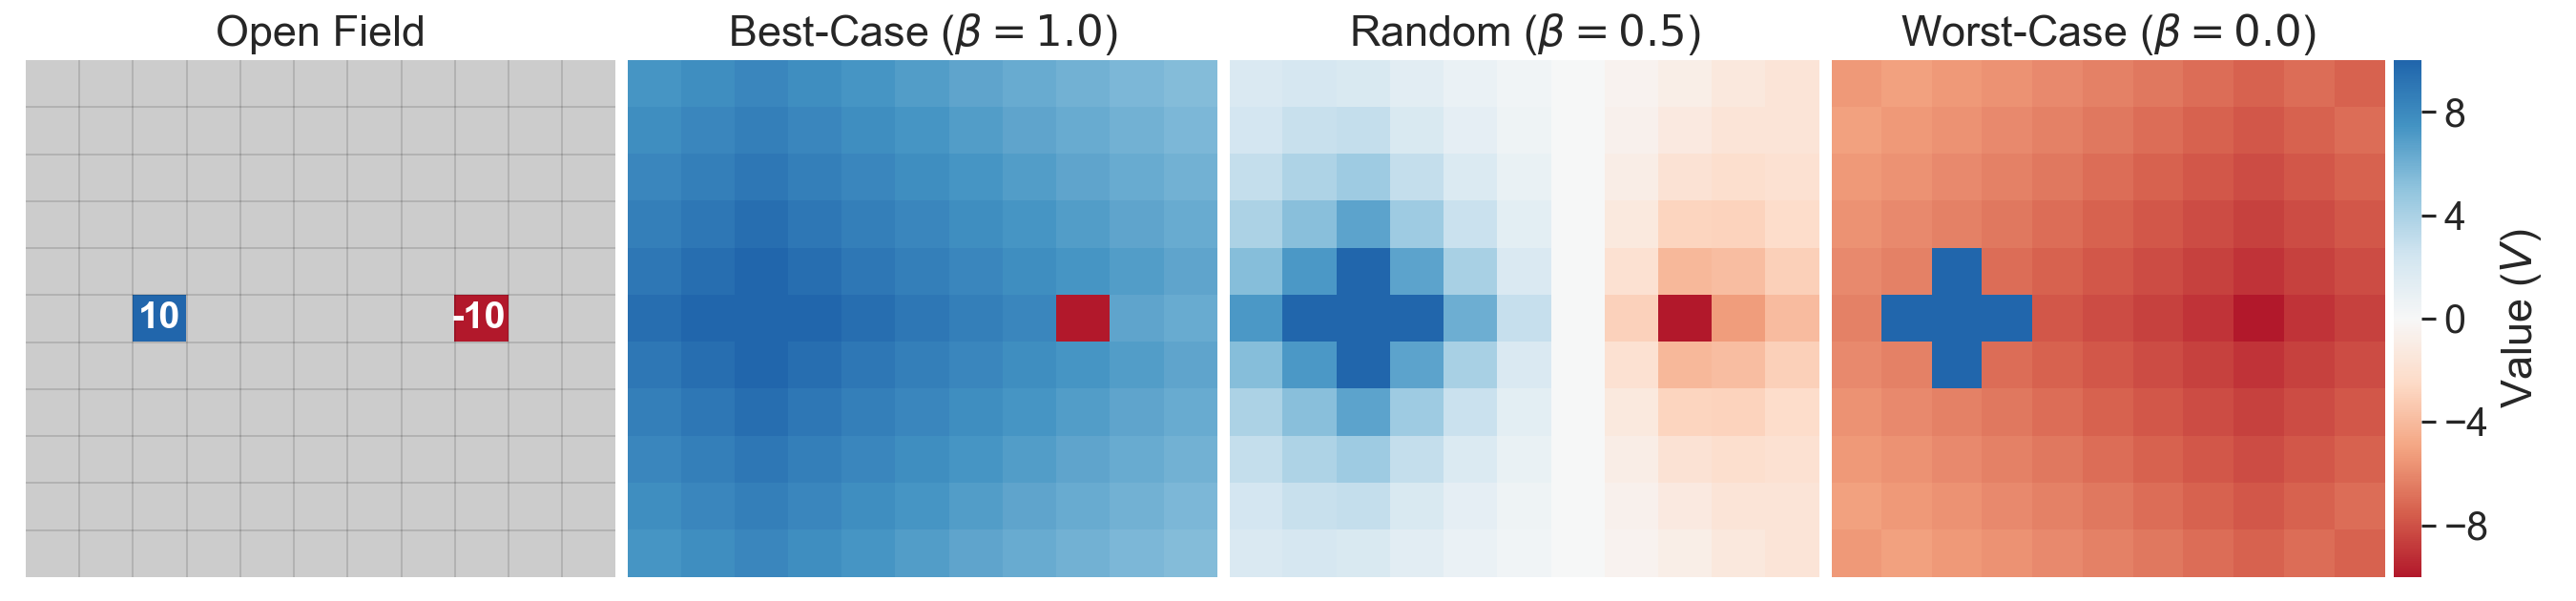
\includegraphics[trim={0 0 0 0},clip]{../figures/01_field.png}}%
  }
  \caption{\textbf{Open Field}}
  \par remember to add parameters
\end{figure}

\subsection{Avoidance}

\begin{figure}
  \centerline{%
    \resizebox{1.0\textwidth}{!}{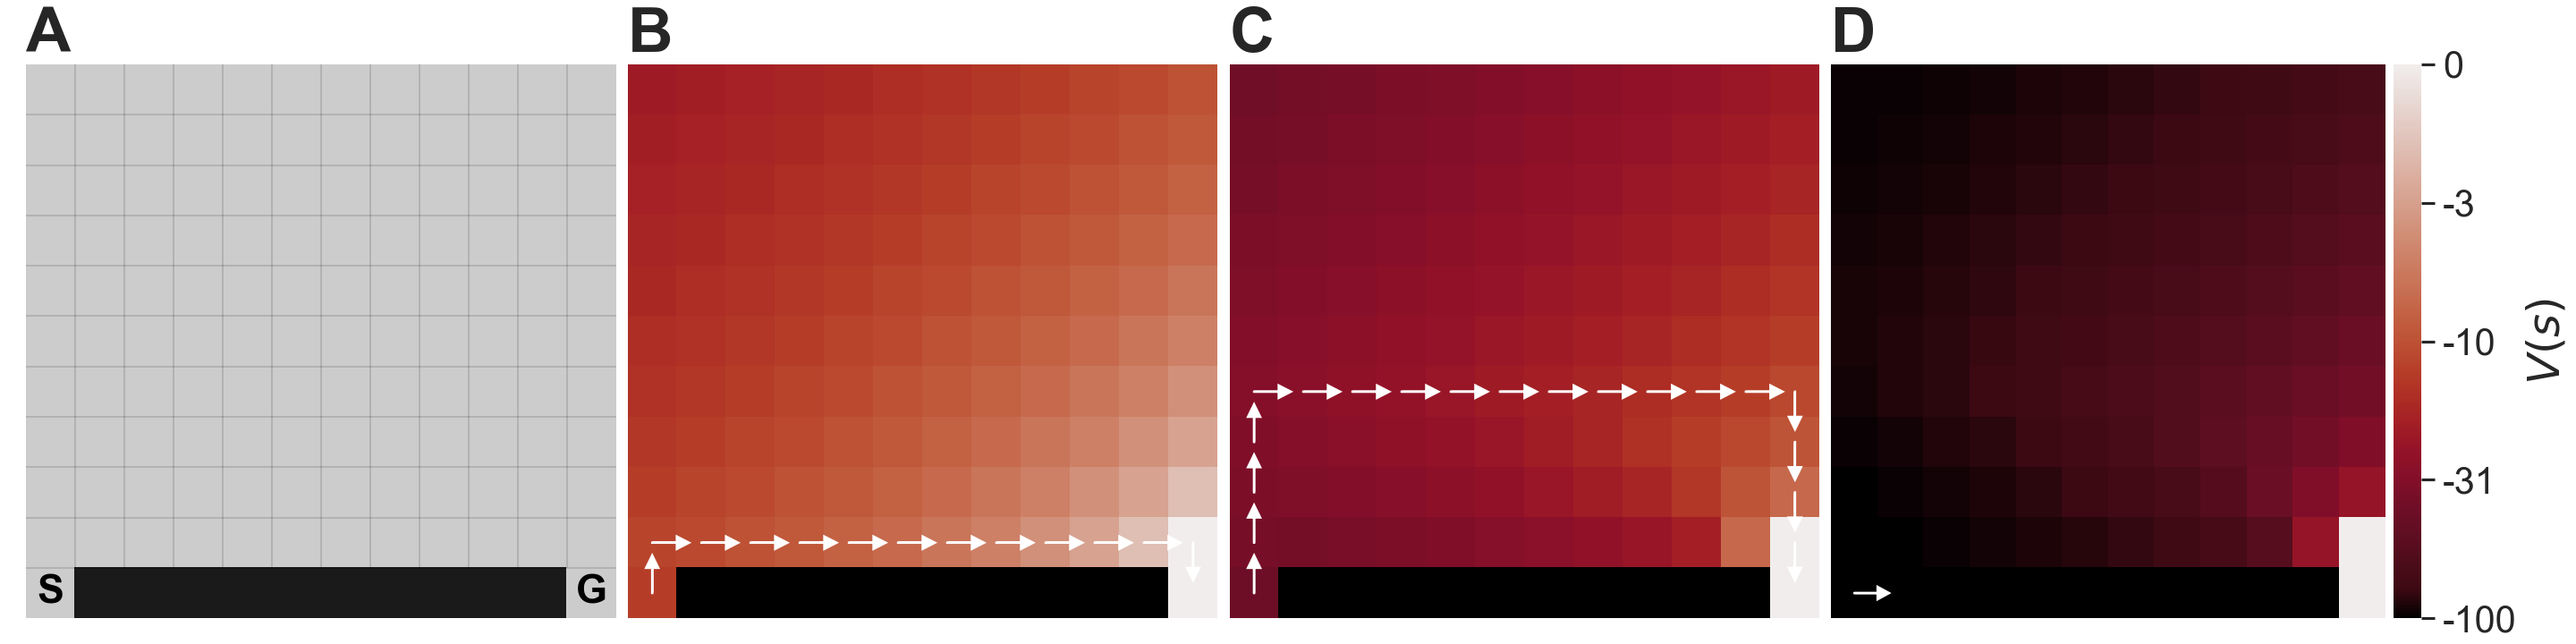
\includegraphics[trim={0 0 0 0},clip]{../figures/02_cliff.png}}%
  }
  \caption{\textbf{Cliff Walking}}
  \par remember to add parameters
\end{figure}

Discuss similar observations in other tasks (Bach et al., 2014; Sheynin et al., 2015).

\subsection{Approach-Avoidance Conflict}

\begin{figure}
  \centerline{%
    \resizebox{1.0\textwidth}{!}{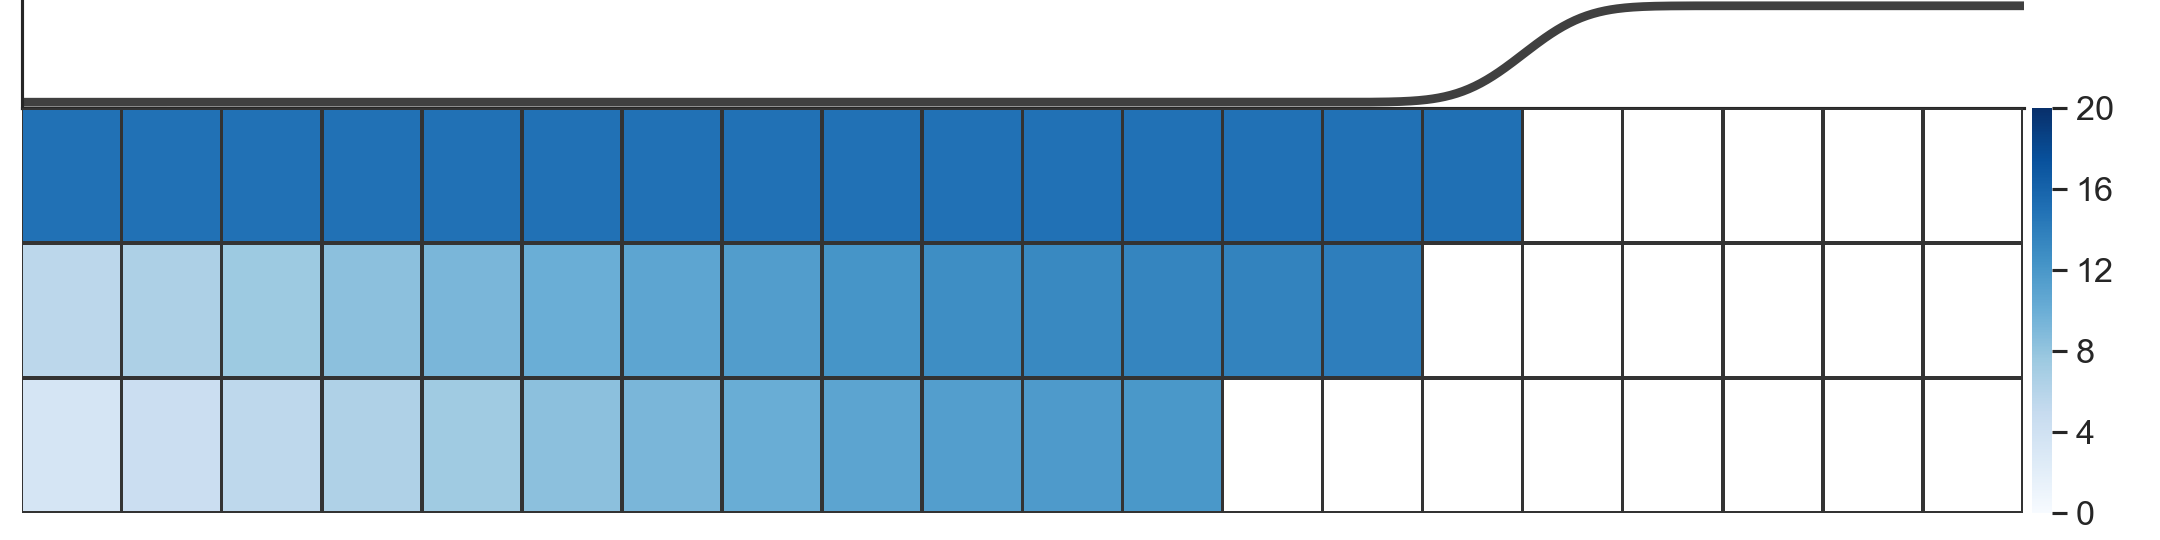
\includegraphics[trim={0 0 0 0},clip]{../figures/03_fid.png}}%
  }
  \caption{\textbf{Flight Initiation Distance}}
  \par remember to add parameters
\end{figure}

Discuss Bach behavioral inhibition.

\subsection{Planning}

\begin{figure}
  \centerline{%
    \resizebox{1.0\textwidth}{!}{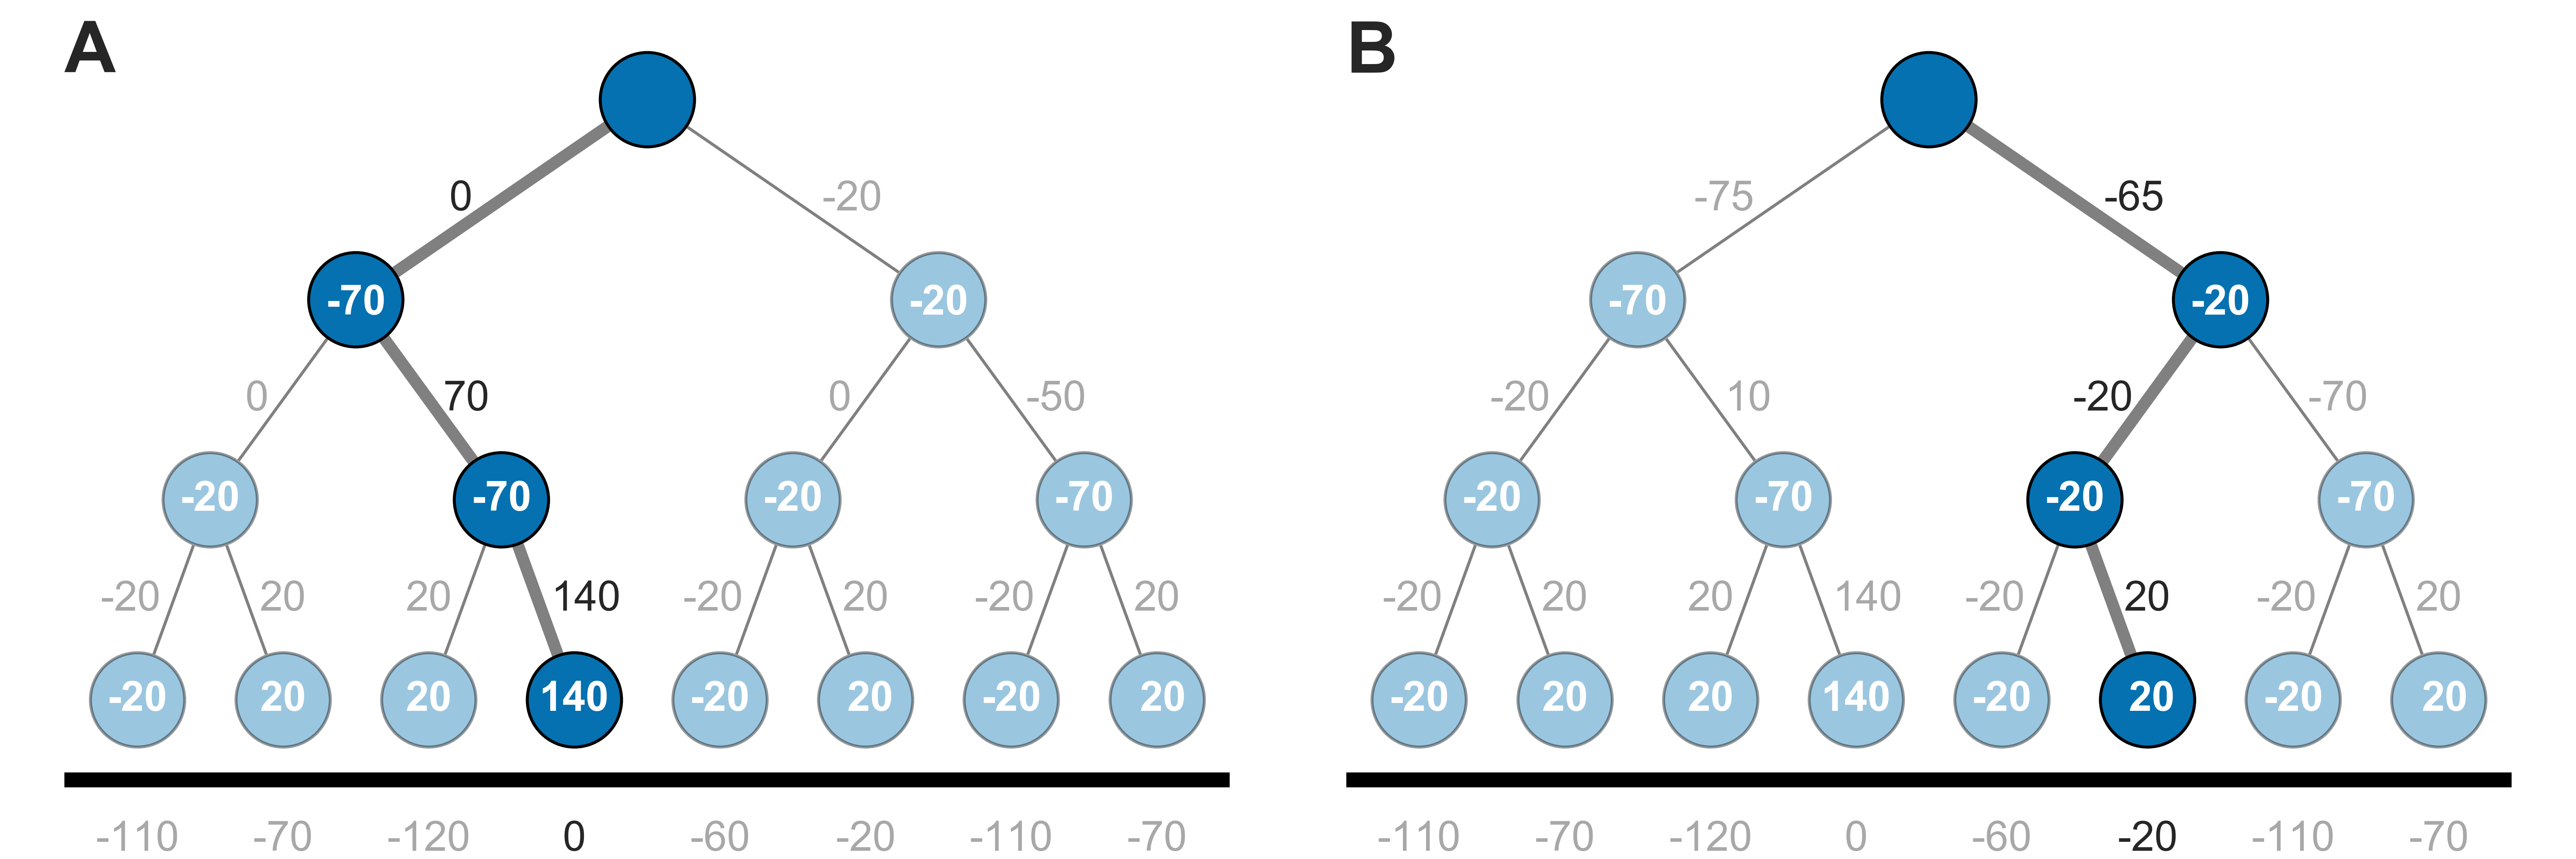
\includegraphics[trim={0 0 0 0},clip]{../figures/04_tree.png}}%
  }
  \caption{\textbf{Decision Tree}}
  \par remember to add parameters
\end{figure}

\subsection{Free Choice Premium}

\begin{figure}
  \centerline{%
    \resizebox{1.0\textwidth}{!}{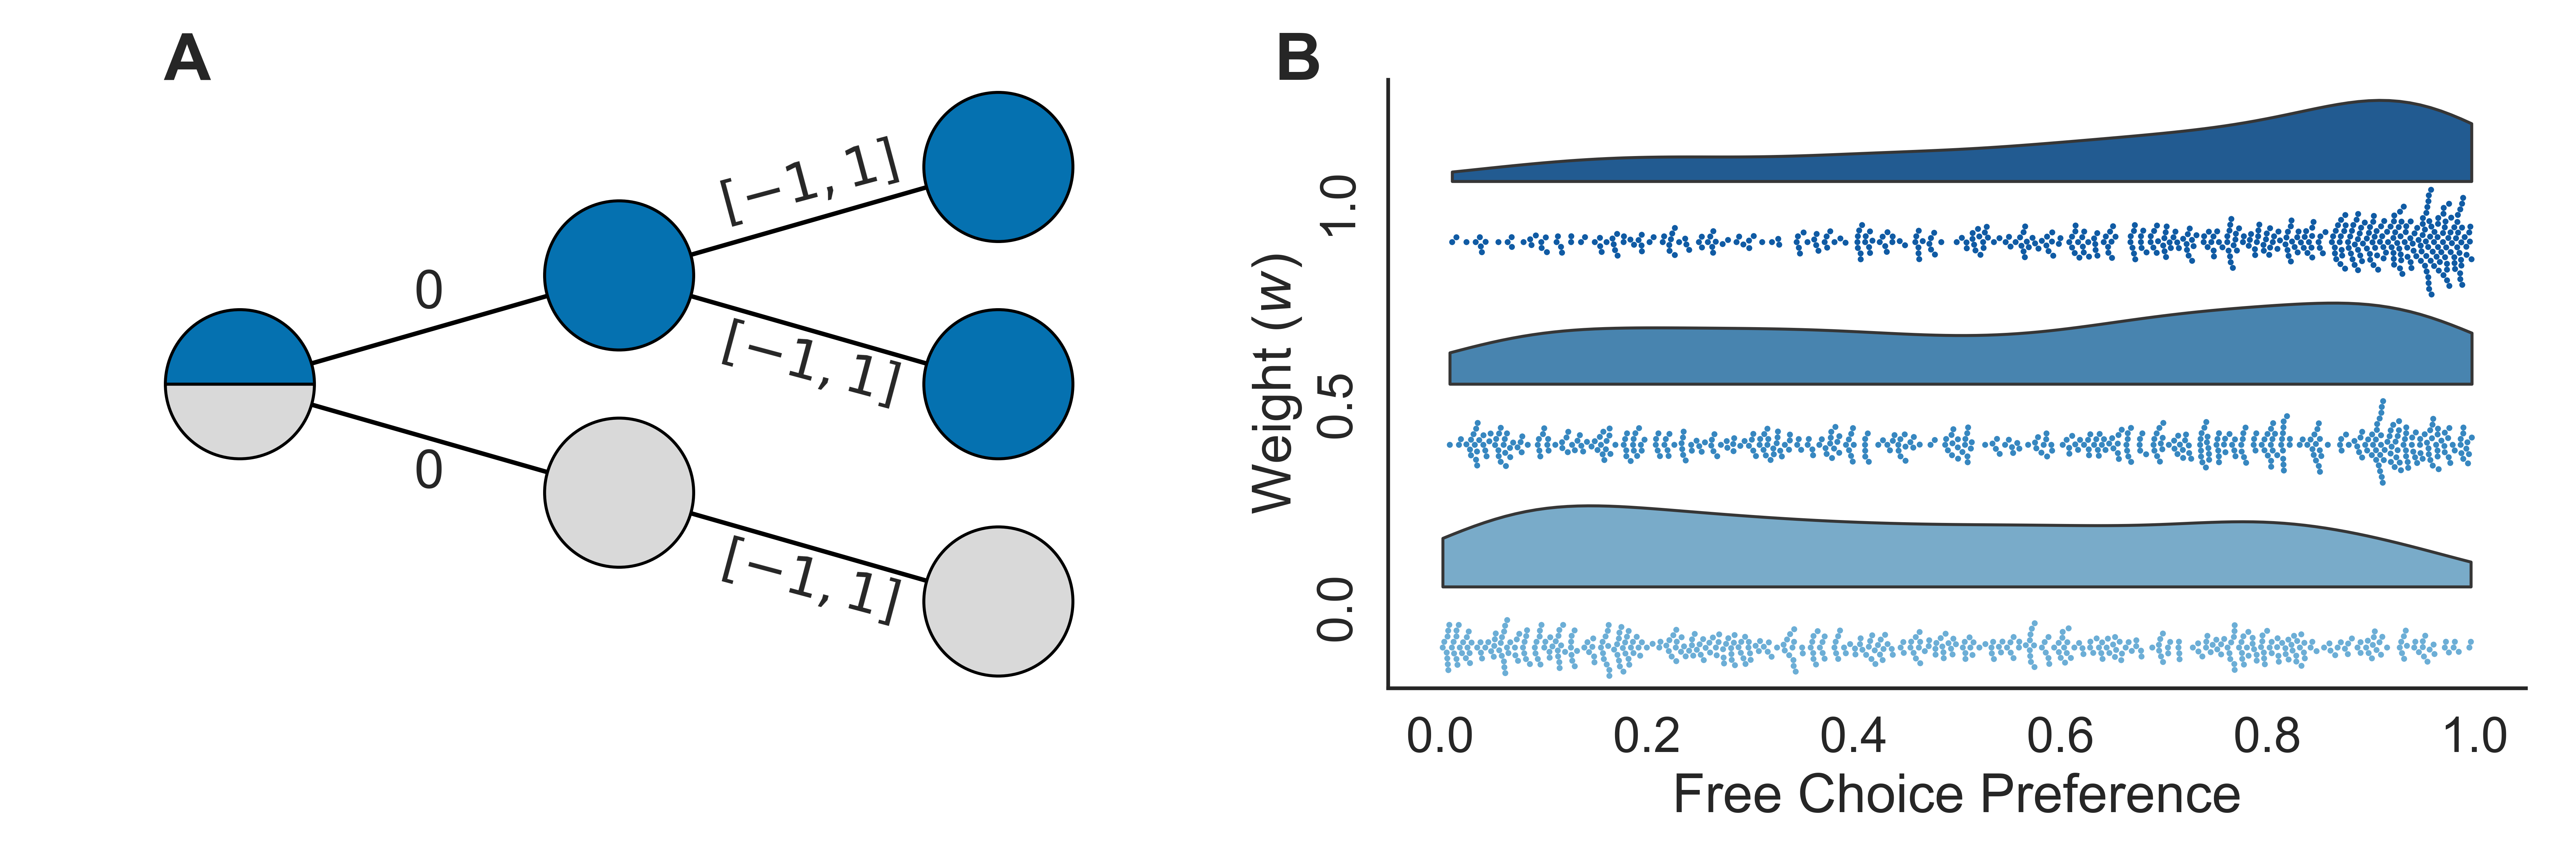
\includegraphics[trim={0 0 0 0},clip]{../figures/05_choice.png}}%
  }
  \caption{\textbf{Free Choice Premium}}
  \par remember to add parameters
\end{figure}

\subsection{Longitudinal Progression}

\section{Discussion}

In this article, we showed...

Discuss previous computational approaches: This has also been previously been
investigated in previous computational modeling \cite{Huys2009}. There
the authors found that beliefs about a lack of controllability, mechanistically
modeled as corrupted priors about action-outcome contingencies, found deficient
learning in novel environments. The present results are no doubt related, but
address a different environment and a different behavior.

We discussed two mechanisms by which negative values can spread. There is a third
that we did not address here: that of the state itself. Here we assumed that states
were fully observable; in other words, there was no uncertainty about the state
an agent was currently occupying. In partially-observable Markov decision problems,
the state itself must be inferred from external and internal variables. This is
yet another means by which bad value can spread if undue likelihood is granted
to undesirable or aversive states. This ideas has previously been proposed to
explain some symptoms in anxiety \cite{Paulus2012}, and not without good reason.
Anxiety disorders involve negatively biased interpretation of ambiguous percepts
\cite{Hartley2012}, which may result in aberrant planning and increased avoidance
for similar reasons to those described above. This is an area for future research.

In this article, we have explored a computational principle of approach and
avoidance learning in sequential decision environments. We have not discussed,
however, the particular psychological or neurobiological mechanisms by which this
sort of learning may take place. This issue has been discussed in detail elsewhere
\cite{Bishop2018}, but we briefly discuss a few possibilities here. Mechanically,
we understand that complex decision problems are solved by mental processes that
exist on a spectrum between model-based and model-free (Daw et al., 2005). The
difference between these two families of methods hinges on the reliance of an
internal model of the world used to make predictions about expected long-run
outcomes of particular choices.

For model-based decision making, one possibility is biased planning. In large
state spaces, online sequential decision making suffers from the curve of
dimensionality: in planning a series of actions to take, comparing between
multiple options rapidly becomes computationally intractable when the number of
options and depth of search becomes even moderately large. Thus, heuristics for
reducing the size of this search can be useful. Biased pruning of search paths
(such as immediately discarding paths that require some minor loss in pursuit of
larger gains) may result in maladaptive decision making (Huys et al., 2012).
Alternately, if planning relies on internal sampling from previously experienced
episodes in order to make predictions about future value, then biased sampling
 may similarly result in maladaptive decision making. Recent work has shown how
 finite sampling during planning can result in risk aversion and the overrepresentation
 of low probability but strongly negative outcomes (Lieder et al., 2018). Such a
 mechanism is prima facie in line with results showing the availability in memory
 of negative outcomes being higher for patients with anxiety (Borkovec et al., 1999;
 Miranda and Mennin, 2007).

Within the realm of model-free decision making, several studies have found evidence
suggesting increased learning rates for negative reward prediction errors in
individuals with elevated levels of anxiety \cite{Aylward, Huang2017, Harle2017
garrett2018}. Though an asymmetry in sensitivity to
positive and negative reward prediction errors bears superficial similarity, for
the reasons described above merely attending more to negative information does not
necessarily predict increased avoidance insofar that avoidance can successfully
isolate negative outcomes. One possibility, and topic of future research, is how
prior beliefs about the reward statistics of the current environment dictate
learning rates. A second possibility is prioritized replay (Russek et al., 2017;
Mattar and Daw, 2018). Offline replay of previous experiences (through hippocampal
mechanisms) are known to facilitate learning. It has been proposed that biased
replay could bias value estimates (Gagne et al., 2018). This is another exciting
area for future research.


\section{References}

\bibliographystyle{authordate1}
\bibliography{citations}

\section{Appendix}
\subsection{Algorithms}

\begin{algorithm}
  \caption{Value Iteration}

  \State Algorithm parameter: a small threshold $\theta > 0$ determining accuracy of estimation
  \State Initialize $V(s)$, for all $s \in S$ arbitrarily, except that $V(terminal) = 0$
  \State
  \While{$\Delta > \theta$}
    \State $\Delta \leftarrow 0$
    \Loop \ for each $s \in S$
      \State $v \leftarrow V(s)$
      \State $ V(s) = \max_a \sum_{s',r} p(s',r|s,a) \left[ r + \gamma V(s') \right] $
      \State $\Delta \leftarrow \max(\Delta, |v - V(s)|)$
    \EndLoop
  \EndWhile

\end{algorithm}

\begin{algorithm}
  \caption{Betamax Temporal Difference Learning}

  \State Algorithm parameters: step size $\eta \in (0, 1)$, small $\epsilon > 0$
  \State Initialize $Q(s,a)$, for all $s \in S$, $a \in A$ arbitrarily, except that $Q(terminal,\cdot) = 0$
  \State
  \Loop \ for each episode
    \State Initialize $S$
    \While{$S \notin S(terminal)$}
      \State Choose $A$ from $S$ using policy derived from $Q$
      \State Take action $A$, observe $R, S$
      \State $Q(S, A) \leftarrow Q(S, A) + \eta \left[ R + \gamma \max_a Q(S',a) − Q(S, A) \right] $
      \State $S \leftarrow S'$
    \EndWhile
  \EndLoop

\end{algorithm}

\end{document}
